\chapter{Alignments with Pair HMMs}\label{CHAPTER:PAIRHMM}

In this chapter we will describe scoring schemes for pairwise sequence alignment
using pHMMs or GpHMM. Scoring schemes used in various programs can differ the
model they use but also in the decoding algorithm. 
We have discussed the use of pHMMs for sequence alignment in section
\ref{SECTION:PAIRHMM}, where we demonstrated  simple three-state pHMM (figure
\ref{FIGURE:SIMPLEPHMM}) that is equivalent to the
Needleman-Wunsch algorithm \cite{Durbin1998}.  First we 
describe three existing  decoding methods for decoding pHMMs.
The rest of the chapter describes several uses of pHMMs and GpHMM in sequence
alignment or in related problems.

Recall from section \ref{SECTION:PAIRHMM} that a pair HMM generates two
sequences simultaneously and that from state path we are able to recover
annotation.


%In following sections we will review several pHMMs and GpHMMs that were used to
%sequence alignments or other purpose, for example gene finding. We will review
%the application domain of the model, its topology, decoding function, parameter
%estimation and optimisation heuristics. But at first, we have to introduce small
%biological background.

\section{Decoding Methods}

In this section we review three decoding methods that were used in literature to
reconstruct pairwise alignments: the Viterbi algorithm, the Posterior
decoding and the Marginalized posterior decoding.

Let $H$ be an pHMM (or GpHMM) and $X$ and $Y$ be the sequences that we want to
align. The probability $\prob{X,Y\mid H}$ is the probability that $X$ and $Y$
were generated in model $H$.  From state path $\pi$ in a pHMM  we can
reconstruct a unique alignment $A_{\pi}$. The model defines the probability 
that
$A_{\pi}$ is the true alignment of $X$ and $Y$ under the assumption, that $X$ and $Y$ were
generated by model $H$:
  \[\prob{\pi\mid
X,Y,H}=\frac{\prob{\pi,X,Y\mid H}}{\prob{X,Y\mid H}}\]
  We can use $\prob{\pi\mid X,Y,H}$ as a score of 
alignment $A_{\pi}$. Path $\pi$ with the highest score can be found by a
two-dimensional version of the Viterbi
algorithm (section \ref{SECTION:PAIRHMMVITERBI}). Alignment $A_{\pi}$ can be
constructed from $X,Y$ and $\pi$ in a straightforward
way: for every match state from $\pi$ that generated $X[i]$ and $Y[j]$ we add
column $(X[i],Y[j])$. For every indel state in $\pi$ that generates $X[i]$ we
add to alignment column $(X[i],'-')$. An indel states for the second sequences are
analogous.  The two-dimensional Viterbi algorithm is used in  most of the
software tools we will discuss later.

Alternatively, we can decode pHMMs using a variant of Posterior decoding.  Two
variants of the Posterior decoding for the pHMMs were described in the
literature: the Posterior decoding and the Marginal posterior decoding
\cite{Lunter2008}.  Let $\prob{X[i]\sim Y[j]\mid X,Y,H}$ be the probability that
$X[i]$ and $Y[i]$ are aligned: the sum of the probabilities of all alignments
that
contain column $(X[i],Y[i])$. Let $\prob{X[i]\sim -_j\mid X,Y,H}$ be the
probability that $X[i]$ is aligned to a gap that is in $Y$ between positions $j$
and $j+1$. Similarly let $\prob{-_i\sim Y[j]\mid X,Y,H}$ be the probability that $Y[j]$
is aligned to a gap in $X$ between positions $i$ and $i+1$. Finally, let
$\prob{X[i]\sim - \mid X,Y,H}$ be the probability that $X[i]$ is aligned to a
gap at any position and let $\prob{-\sim Y[j]\mid X,Y,H}$ be the probability
that $Y[j]$ is aligned to a gap at any position.  Posterior probabilities
defined above can be computed by the two-dimensional version of the
Forward-Backward algorithm (probability that a symbol is aligned to a gap at any position
is the sum of the probabilities that symbol is aligned to a gap at position $i$
for all possible positions $i$).

Let alignment $A$ of sequences $X$ and $Y$ have length $n$ and
consists of columns $a_0,a_1,\dots a_{n-1}$. Each column is a pair
$a_i=(x_i,y_i)$ where $x_i$ and $y_i$ are symbols from $\Sigma\cup\{-\}$ \footnote{Note that $x$ and $y$ cannot be both gap symbols.}.
Let $d_A^x(i)$ be the number of non-gap symbols in $x_0,x_1,\dots x_{i}$,
let $d_A^y(i)$ be the number of non-gap symbols in $y_0,y_1,\dots, y_{i}$ and
define $d_A^x(-1)=d_A^y(-1)=0$. In this notation, $A[0:i]$ is an alignment of $X[:d_A^x(i)]$ 
and $Y[:d_A^y(i)]$. Then the posterior probability of an alignment column $a_i$ is
\[P(a_i)=
\begin{cases}
\prob{x_i\sim y_i\mid X,Y,H} & \text{if $x_i$ and $y_i$ are not gap symbols}\\
\prob{x_i\sim -_{d_A^y(i)-1}\mid X,Y,H}  & \text{if $y_i$ is gap symbol and $x_i$ not}\\
\prob{-_{d_A^x(i)-1}\sim y_i\mid X,Y,H}  & \text{if $x_i$ is gap symbol and $y_i$ not}
\end{cases}
\]

The \abbreviation{Posterior decoding}{PD} finds the alignment $A$ that maximizes
the product of the posterior probabilities of its columns: 
\[A = \arg\max_{A'\in Al(X,Y)}\prod_{0\leq i <
|A'|}P(a'_i)\] where $Al(X,Y)$ denote the set of all  alignments of sequences
$X$ and $Y$. Similarly we can define \abbreviation{Marginalized posterior
decoding}{MPD}: Let $P'(a_i)$ be the marginalized posterior probability:
\[
P'(a_i) = \begin{cases}
P(a_i) & \text{if $x_i$ and $y_i$ are not gap symbols}\\
\sum_{0\leq j < |Y|}\prob{x_i\sim -_{j}\mid X,Y,H}  & \text{if $y_i$ is gap symbol and $x_i$ not}\\
\sum_{0\leq j < |X|} \prob{-_{j}\sim y_i\mid X,Y,H}  & \text{if $x_i$ is gap symbol and $y_i$ not}
\end{cases}
\]
Then the MPD finds an alignment $A$ that maximizes the product of the
marginalized posterior probability:
\[A = \arg\max_{A\in Al(X,Y)}\prod_{0\leq i < |A'|)}P'(a'_i)\] 

The Posterior decoding and the Marginalized posterior decoding were used by
Lunter {\it et al.} and both produced better alignments than alignments found
by the Viterbi algorithm (more details in section \ref{SECTION:BIASES}). Once posterior probabilities of all possible columns of an
alignments are computed (in $O(|X||Y|k^2)$ time where $k$ is the number of
states of pHMM), we can find the alignment that maximizes the desired
function in $O(|X||Y|)$ time \cite{Lunter2008}. 

%Other decoding method can be done by the poster
%Other option is to
%use the  Posterior decoding: for every pairs of residues $X[i],Y[j]$ we compute
%posterior probability that $X[i]$ and $Y[j]$ are aligned $\prob{X[i]\sim Y[j]\mid X,Y,H}$.
%Score of an alignment is sum of posterior probabilities of the aligned residues.
%Later in this chapter we show different variants of the Posterior decoding for
%pHMM.


\section{Pair Hidden Markov Models with Gene Structures}

In this section we describe several pair hidden Markov models (or generalized
pair hidden Markov models) with gene structures incorporated into their
topology. These models were used either to align coding DNA or proteins
to a genome or to find genes.


First we introduce several comparative gene finders. Comparative gene finders
use evidence from two organisms to find genes. They use pHMM to simultaneously
align and annotate the two sequences. The advantage finding genes in two
organisms simultaneously is that we can use the evidence from two related
organisms to detect genes that are in both organisms.

\subsection{DoubleScan}
Meyer {\it et al. (2002)} developed comparative gene finder DoubleScan.
Generally, DoubleScan has three types of states: {\it match} states, which
generate same number of symbols in both sequences;   {\it emit} states, which
generate sequences only in one sequence and silent states.  

The basic structure of DoubleScan's GpHMM consists of three types of
substructures: substructures that emits exons, substructure that emits introns
and substructure that generate intergenic regions. Each structure has three
copies in the model: one for match states and two for emit states. Exon
substructure is a single state emitting codons (triplets that will be translated
into amino acids).  There is one additional intron substructure connected to
states that generate intergenic regions. This additional intron substructure is
in the model to avoid detecting of pseudogenes. The GpHMM has $54$ states.

%Every such
%structure has three version: one matching version, which emit aligned residues
%and one structure per sequence to emit indels.  Overview of DoubleScan's HMM
%structure is in figure \ref{}. 
\nocite{Meyer2002}

Emission probabilities of the {\it match exon} state were estimated from
relative frequencies in the training set with Dirichlet priors
\cite{Meyer2002,Durbin1998}.  Emission probabilities of other states were
generated  by marginalizing emissions of the match exon state. Transition
probabilities from the initial state were uniform, transition probabilities for
splice sites were estimated by splice site predictor. Other transitions were
observed from training data and tuned by hand.

DoubleScan uses the Viterbi algorithm as a decoding method.  To reduce the
running time of the Viterbi algorithm they use stepping-stone algorithm: first
they run BLASTN to find local alignments. Then DoubleScan chooses a consistent
subset of alignments by the greedy method described in section
\ref{SECTION:SSA}. They restrict the Viterbi algorithm to follow the alignments
in the subset allowing tolerance 15 bases.

\subsection{SLAM} 

\begin{figure}
\begin{center}
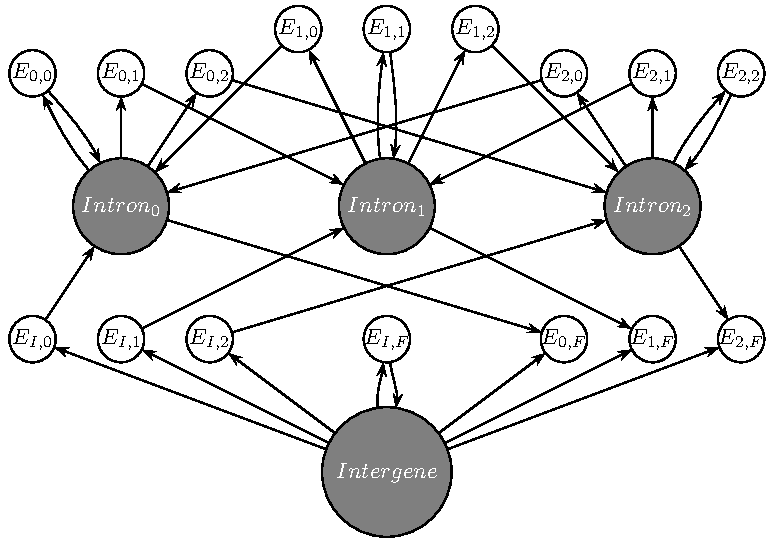
\includegraphics{../figures/slam.pdf}
\end{center}
\caption[HMM topology of SLAM's GpHMM]{
Topology of GpHMM used by SLAM (states for genes on reverse strand are omitted).
Gray states have geometric distribution (modeled with self-loops which are
omitted in the figure). Emissions of shaded states are modeled by the basic
three state pHMM. White states represent exons. Each has associated a duration
distribution and emissions are also modeled by three-state pHMM using $5$-th
order states that emit whole codons at once.  Since introns can be inside a
codon, the model contains an exon state for every possible interruption:
$E_{i,j},0\leq i,j<3$ is an exon that begins with end of the interrupted codon of
length $((3-i)\mod 3)$ and ends with the start of a codon of length $j$. $I$
stands for start codon and $F$ stand for stop codon: states
$E_{I,\cdot},E_{\cdot,F}$ and $E_{I,F}$ model exons adjacent to the beginning
and the end of a gene.  $Intron_i$ models intron that interrupted codon at the
$i$-th position ($0$ means that intron is not interrupting any codon).
}\label{FIGURE:SLAM} \end{figure}

SLAM \cite{SLAM2003}  is a comparative gene finder based on a generalized pair
hidden Markov model \cite{Alexanderson2004} with some states being also
high-order states (with dependence on previous emissions).  It predicts gene
structures for a pair of related eukaryotic organisms. SLAM's decoding method is
the Viterbi algorithm. 

Unlike DoubleScan, SLAM defines a true GpHMM because state durations are not
constant, but are sampled from some distribution (however, distribution they
used is not specified). Topology of the model can be found in figure
\ref{FIGURE:SLAM}.  Emission probabilities of pairs of codons were assigned from
a codon-based PAM matrix.


To reduce the running time of the algorithm first they  align the input
sequences using AVID global alignment tool \cite{Bray2003}. They restrict the
Viterbi algorithm so, that each base matched in the anchor alignment can be
realigned in an interval of size $3$.

\subsection{TWAIN}

TWAIN is another approach to use GpHMM to find genes \cite{Majoros2005} and is
interesting because of its decoding algorithm. Twain GpHMM has two types of
states: the states with fixed durations (which emit sequences of fixed length)
and the states with variable duration lengths which are associated with some
distribution.  The states with fixed durations corresponds to specific
signals, such as splice sites, start/stop codons, and so on.
Additionally, the states with variable duration are not connected with each
other; the transitions from/to such states are only to/from states with fixed
duration lengths. Therefore if we know the positions of all signals in the
sequence, we know that sequences between signals were generated by one state.
This can be exploited in the following way.

TWAIN at first annotates input sequences using gene-finder TIGRscan
\cite{Majoros2004} (each sequence is annotated independently) which finds
signals in the sequences and creates a parse graph: vertices of the parse graph are
the signals in the sequence (each signal corresponds to a state of the GpHMM).  Two
signals are connected with an edge if in the genome one signal can follow another:
for example a start codon can be followed by a stop codon or a donor site.
Therefore start codons are connected with following stop codons and
donor sites. Each edge is scored by the probability of the most probable state
path between those two states in the TIGRscan's HMM. To reduce the size of the
graph, some edges are omitted by heuristic.

TWAIN creates graph $G$ by cartesian product of two parse graphs and omits the
vertices that corresponds to pairs of different signals since they are unlikely
to be seen in the alignments. Each node in the graph corresponds to some state $s$
of the GpHMM and cell $c$ in the dynamic programming matrix of the Viterbi
algorithm.   Edges between cells $c_1,c_2$ correspond to alignments
generated by a single state from GpHMM (since states for $c_1$ and $c_2$ are
connected through generalized states).  The Viterbi algorithm is computed only
on cells corresponding to graph $G$ which significantly reduces running time
\cite{Majoros2005}.


\subsection{GeneWise}

GeneWise predict genes by aligning a protein  to similar gene structures in DNA
\cite{GeneWise2004}. Instead of pHMM defined as in section \ref{SECTION:PAIRHMM}
it uses probabilistic transducers. Probabilistic transducers are very similar to
pHMM. They are both probabilistic finite state machines, but unlike pHMMs which
generate two sequences, probabilistic transducers transform one sequence into
the other sequence.  The second difference is that transducers have emissions
associated with transitions, not with states.  Therefore transducer emission of
the form $e_{u\to v,(x,y)}=p$ means that during transition $u\to v$ symbol $x$
is read from the input sequence and symbol $y$ is written to the output with
probability $p$ ($x$ or $y$ might also be the gap symbol).  While pHMMs defines
distribution $\prob{X,Y\mid H}$, probabilistic transducers define distribution
$\prob{X\mid Y,H}$, the probability that sequence $Y$ will be transformed to
sequence $X$.

Advantage of transducers over the pHMM is that we can easily compose multiple
transducers together, while maintaining probabilistic interpretation of the
resulting model.  Composition of two transducers $A$ and $B$ is transducer $C$
that transforms sequence $X$ to some sequence $Y$ using transducer $A$ and then
transforms $Y$ to sequence $Z$ using transducer $B$. 

GeneWise model was created by composition of a gene prediction model $S$ which
translates genomic sequence to protein sequence and a protein homology model $T$
which maps protein sequence to a homologous protein sequence.

Gene prediction model $S$ consists of a single exon state which translates
series of codons into amino-acids. It has three submodels for modeling introns,
each consisting of $3$ states representing  splice sites, poly-pyrimidine tract
and central intron section (those $3$ states are associated with $4$
transitions, each transition emit one feature). 

Protein homology model $T$ is a simple pHMM from figure \ref{FIGURE:SIMPLEPHMM}
defined over protein alphabet.  The composition of the models $T$ and $S$ has
$30$ states. Authors removed unnecessary states and they also removed
poly-pyrimidine states to reduce the number of states and transitions
\cite{GeneWise2004}.


\subsection{Pairagon}

\begin{figure}
\begin{center}
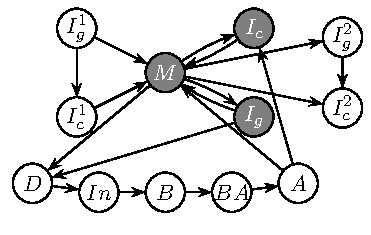
\includegraphics{../figures/pairagon.pdf}
\end{center}
\caption[Topology of Pairagon generalized pair hidden Markov model.]{
Topology of Pairagon GpHMM. All states except states
$D,B$ and $A$ have a self-transition.
Shaded states corresponds to exons: $M$ emits
aligned pairs of symbols, $I_c$ is insertion in the cDNA and $I_g$ is
insertion in the genome. States $I^1_c,I^1_g,I^2_c$ and $I^2_g$ corresponds to
unaligned parts of the DNA and cDNA in the beginning and the end of the
sequences. States $D,In,B,BA,A$ corresponds to intron structure and stand for 
Donor, Intron, Branch, Branch Acceptor and Acceptor respectively.
Donor site emits $8$ symbols and acceptor site emits $6$ symbols.
}\label{FIGURE:PAIRAGON}
\end{figure}


The aim of Pairagon is to find local alignments of \abbreviation{complementary
DNA}{cDNA} and genome \cite{Pairagon2009}. By aligning experimentally obtained
cDNA sequences to the genome we are able to confirm intron and exon structures
of genes.  Pairagon's HMM model consists of a simple pair HMM submodel, which
aligns cDNA to DNA and a $5$-state submodel for intron structures. The whole
topology is in figure \ref{FIGURE:PAIRAGON}. 

Model was trained using iterative maximum likelihood approach.  Initial
parameters were trained on the alignments from the \abbreviation{Mammalian Gene
Collection}{MGC}. In this phase, the parameters for intron submodel were set by
hand. The model was then used to align more MGC sequences. Final parameters were
estimated from the new alignments.

Decoding was done by the Viterbi algorithm. Runtime of the algorithm was
improved by the stepping-stone algorithm described in section \ref{SECTION:SSA}
and memory requirements were improved using the Treeterbi algorithm
\cite{Keibler2007}, which is similar to the On-line Viterbi algorithm discussed
in section \ref{SECTION:ONLINEVITERBI}.


\section{Non-Geometric Indel Models}
In the simple pHMM described in figure \ref{FIGURE:SIMPLEPHMM}, gap length has
geometric distribution: the probability that a gap has length $n$ is
$e_{M,I}e_{I,I}^{n-1}(1-e_{I,I})$ (note that the probability that at particular
position will be gap with length zero is $1-e_{M,I}$). The Viterbi
algorithm is usually computed in log-space: instead of computing product of
probabilities of events\footnote{Event is emission or transition.}, we compute
the sum of logarithms of those probabilities, because computation in log-space
is numerically more stable. The Viterbi algorithm for the simple HMM
will become the same as the Needleman-Wunsch algorithm.  Gap penalty will be
$\log(e_{M,I})+\log(1-e_{I,I})+(n-1)\log(e_{I,I})$. By setting $d=\log(e_{I,I})$
and $g=\log(e_{M,I})+\log(1-e_{I,I})-d$ we see that this is exactly affine gap
penalty. Therefore we can say that affine gap penalties correspond to geometric
distribution of indel lengths.

As we mentioned in chapter \ref{CHAPTER:ALIGNMENT}, using non-affine gap model
can improve alignment quality.  Problem with geometric distribution (or affine
gap penalties) it that they are not realistic \cite{Cartwright2009,Lunter2008}.
Therefore some other distribution might be more appropriate, for example zeta
distribution \cite{Cartwright2009}, or combination of several geometric
distributions to approximate the distribution of gap length
\cite{Gill2004,Gill2006}.

GpHMM allow us to use arbitrary duration distributions.  On the other hand,
GpHMM are much slower to decode.  One way of incorporating a different gap
distribution into pair hidden Markov models without using their generalized
version is to use several (for example two) indel states for every sequence. For
example Lunter {\it et al. (2008)} used two component mixture models: instead of
one indel state for every sequence they use two. They report that this improved
quality of alignments. Similar approach is used in the multiple sequence aligner
FASTA \cite{Bradley2009}. \nocite{Lunter2008}

Modeling non-geometric distributions with several states can be problematic when
used with the Viterbi decoding \cite{Vinar2005}. Set of states with the same
emission distribution used for modeling non-geometric distribution is called
gadget. We discuss an example of such a problem for the two component mixture
model.

\begin{figure}
\begin{center}
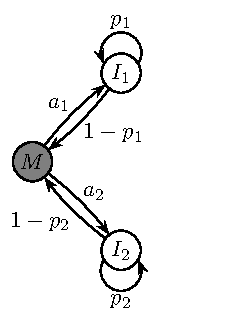
\includegraphics{../figures/twoComponentMixtureModel.pdf}
\end{center}
\caption[The example of an HMM modeling two component geometric distribution]{
Shaded state $M$ represents the match states and states $I_1$ and $I_2$
represents indel states in the same sequence. Indel states for the other
sequence are omitted.
}\label{FIGURE:TWOCOMPONENT}
\end{figure}

Let $H$ be a simple pair hidden Markov model with two pairs of indel states.
Let $I_1$ and $I_2$ be indel states that generate gaps in the first sequence
connected with match state $M$ as in the figure \ref{FIGURE:TWOCOMPONENT}.  Gaps
in alignments (in the first sequence) that are generated by such a model have
length distribution $d(n)=(a_1p_1^{n-1}(1-p_1)+a_2p_2^{n-1}(1-p_2)), n>0$ and
$d(0) = 1-a_1 - a_2$ where $n$ is the length of the gap ($n=0$ means that there
is no gap), $a_1$ and $a_2$ are probabilities of entering state $I_1$ and $I_2$
respectively and $p_1$ and $p_2$ are probabilities of remaining in state $I_1$
and $I_2$ respectively.  This is equivalent to the generalized pair hidden
Markov model $H'$ with one indel state for every sequence which has
$d'(n)=d(n)/(1-d(0))$ as its duration distribution (in generalized states we
want to have at least one state. The $d(0)$ should by modeled by the
probabilities of incoming and outgoing transitions). Both models define the same
distribution of alignments  and running the Forward-Backward algorithm or the
Forward algorithm will give the same results. However, alignments constructed by
the Viterbi algorithm can be different for $H$ and $H'$.

Problem is that in the generalized model the Viterbi algorithm gaps of length
$n$ have ``score'' $d(n)$ but in the non-generalized pair hidden Markov model it
will be $m(n)=\max\{a_1p_1^{n-1}(1-p_1),a_2p_2^{n-1}(1-p_2)\}, n>0$ and
$m(0)=1-a_1-a_2$.  These two scores are different ($d(n)$ is always higher) and
therefore it is possible that the Viterbi algorithm reconstruct different
alignments. Therefore if we are using the Viterbi algorithm, we should either
construct a gadget so that $m'(n)$ will be a better approximation of $d(n)$
($d(n)$ is the distribution for the original model) or use a generalized pair
hidden Markov model for the Viterbi algorithm.

%co chcem povedat: niekedy je lepsie pouzit iny gapmodel -- jeden pre kratke
%gapy, jeden pre slhe gapy. Preto sa niekedy 

\section{Aligning Sequences with Variable Rate of Evolution}
\label{SECTION:FEAST} 
%\subsection{FEAST} 

The rate of evolution (the expected number of substitution per position in
sequence over some period of time) is not constant for the whole genome. It does
not have to be constant even within one gene. FEAST is pairwise local alignment
tool \cite{FEAST2011} that takes into account the variable evolution rate. The
simple pHMM from figure \ref{FIGURE:SIMPLEPHMM} is optimized for one fixed rate
of evolution.  FEAST contain $k$ such submodels, each trained for a different
rate of evolution.  Submodels are connected with a single silent state.  Since
FEAST is a local alignment tool, it also contains one additional submodel for
generating an unaligned pair of  sequences  at both ends of the sequences.

To construct an alignment (either local or global) FEAST uses the Viterbi
algorithm. Like many local aligners, FEAST uses a seeding heuristics to reduce
computational complexity of finding local alignments.  At first it uses six
different space seeds to get candidate seed and then extends those seeds using
x-drop heuristic \cite{Altschul1997}. The extension is done by an ungapped
version of the Forward algorithm, in contrast with the Viterbi algorithm usually
used for this purpose. 

Estimation of parameters was done by expectation maximization approach (with
Baum-Welsch or Viterbi training). They forced gap parameters to be the same in all
submodels.

Different rates of evolution were also used  in the whole genome aligner GRAPe
\cite{Satija2010}. GRAPe's HMM  consists of two submodels: one with fast
evolution rate and two component geometric mixture model for indels and one with
the lower evolution rate and geometric distribution of indel lengths. GRAPe uses
the Posterior decoding as a decoding method.


\section{Biases In Alignments}
\label{SECTION:BIASES}
Lunter {\it et al. (2008)} conducted an extensive survey concerning biases in
alignment. They considered three types of biases associated with gaps. These gap
biases are also discussed in \cite{Durbin1998}. By \firstUseOf{true alignment}
we mean an alignment that corresponds to the actual evolution history.  Since
true alignments are unknown for real data we can simulate evolution on randomly
generated sequences, this obtaining a dataset of ``true'' alignments.

\begin{itemize}

\item \firstUseOf{Gap wander} means that a gap is in a different location that in
the true alignment. Is is due to random short similarities around the borders of
gaps that are indistinguishable from true homologies.

\item \firstUseOf{Gap attraction} is occurs when two gaps are near each other.
In such case merging those gaps and introducing a few mismatches might lead to
higher score. 

\item \firstUseOf{Gap anihilation} occurs when there are two gaps of the same
length, one in each both sequence. Since indels are not so common, removing both
gaps while introducing new mismatches might increase the score of an alignment.

\end{itemize}


Biases are ordered by their frequency from the most occurring to the least
occurring \cite{Lunter2008}. Lunter {\it et al.} explore there problems with a
series of simulations.

They measure the alignment quality by \firstUseOf{sensitivity}, which is the
ratio of the correctly predicted alignment columns to all homologous columns in
the true alignment \cite{Lunter2008}. 

In the first experiment, authors use a simple model of evolution obtaining
alignments with the expected sequence identity $0.705$ with geometric gap model.
The sequences were then realigned using the Viterbi algorithm with the same
model as was used for simulation. Sensitivity was lowest for the  columns near
gaps ($56$\%) and the sequence identity for columns near gaps was $85$\% which
does not agree with the expected sequence identity $0.705$\%.  Moving away from
gaps the average sequence identity dropped to  $0.68$\%. The increased sequence
identity near gaps is due to gap wander bias. The gap attraction effect caused
that the number of gaps that are  near each other was lower than the expected
value obtained from the used gap model.

They also run the Viterbi algorithm parametrized by a range of substitution and
indel rates. The highest sensitivity was obtained for the parameters that were
identical to the parameters used for simulation. However, even then the
sensitivity was only $84$\% indicating that even if we have the right evolution
models, some biases in the alignments are inevitable.  

Lunter {\it et al.} also studied the effect of different decoding methods and
different models on the alignment quality. They simulated evolution with
parameters that are close to the parameters of human-mouse evolution. They
simulated for example the large-scale variation of GC content, GC-content
dependent indel and substitution rates and GC-independent local substitution
rate variation \cite{Lunter2008}.  From simulation they obtained $20,000$
homologous sequence pairs with average length of $700$ nucleotides. They add
flanking sequences of length $100$ nucleotides to the generated sequences  to
simulate local alignments.

After simulation they realigned homologous sequences using the Viterbi algorithm
(VA), the Posterior decoding (PD) and the Marginalized posterior decoding (MPD)
with different models: the three state pHMM ($H_S$); $H_S$ with two indel states
for
every sequence  representing the two component geometric mixture gap model ($H_M$) and the
full model with all parameters that were used for simulation ($H_F$).

They also introduce two additional measures of the alignment quality. The
\firstUseOf{false positive fraction (FPF)} is the proportion of the columns that
are ungapped in the true alignment but wrongly aligned by an algorithm
\cite{Lunter2008}. The \firstUseOf{the nonhomologous fraction (NHF)} is the
proportion of columns containing padding sequence among all columns aligned by
an algorithm.


The use of the different models has little impact on the sensitivity of the
constructed alignments. It is interesting that for the Viterbi algorithm the
sensitivity was lower for the full $H_3$ model than for the simple model $H_1$.
This might be explained by the multiple path problem.  With other decoding
algorithms the models $H_2$ and $H_3$ has slightly higher sensitivity then the
$H_1$ model. 

While the use of the ``better'' model does not significantly improve the quality
of alignments, using the Posterior decoding and Marginalized Posterior decoding
improved the sensitivity by approximately $2.5$\% regardless of the model. On
the other hand the FPF and the NHF was increased with use of the PD and MPD. The
sensitivity of the PD and the MPD were similar but the FPF was lower for the MPD
than for PD. 

The main outcome of this experiment is that proper decoding method can improve
the alignment quality while the use of a simpler model doest not significantly
reduce the alignment quality. However, Lunter {\it et al.} use in their
simulations models only relatively simple models of the evolution. By
incorporating information about gene stricture into alignment models combined
with the use of the right decoding algorithm we can improve alignments further.
This will be discussed in the next chapter. 


